\documentclass[a4paper, titlepage]{article}

\usepackage{graphicx}
\usepackage{color}
\usepackage[colorlinks=true, urlcolor=blue, linkcolor=black]{hyperref}
\usepackage{graphicx}

\newcommand*{\email}[1]{\href{mailto:#1}{#1}}
\newcommand*{\uaEmail}[2]{\email{\lowercase{#1}.\lowercase{#2}@student.uantwerpen.be}}
\newcommand*{\nameAndMail}[2]{#1 #2 - \uaEmail{#1}{#2}}

\begin{document}
	\title{Introduction to git\\ \large An initiative for 1BAinf}
	\date{November 13, 2018}

	\author{
		\nameAndMail{Stijn}{Rosaer} \\
		\nameAndMail{Andrei}{Bondarenko} \\
		\nameAndMail{Igor}{Schittekat} \\
		\nameAndMail{Joey}{De Pauw} \\
		\nameAndMail{Senne}{Rosaer} \\
		\nameAndMail{Toon}{Meynen}
	}
	\maketitle
	\tableofcontents
	
	\section{Intro}
		Github is een versiebeheersysteem waar software geplaatst kan worden. Dit houdt in dat men code hier kan plaatsen, updaten, downloaden en terug gaan naar een voorgaande versie. Ook is dit gemakkelijk wanneer men met verschillende personen tezamen werkt aan dezelfde code. We willen zo een overzicht behouden en op een wel bepaald moment elks aan code kunnen werken, zonder dat de code van de ander op dat moment be\"invloed wordt.
	

	\pagebreak
	
	\section{How to use git}
		\subsection{Starting with Github}
			\begin{enumerate}
				\item Om github te gebruiken moeten we eerst een account aanmaken. Ga hiervoor naar \href{https://github.com/}{\textit{github.com}} en cre\"eer een account.\\	
				Gebruik zeker je UA-mailadres (voornaam.achternaam@student.uantwerpen.be), je kan namelijk als student gratis private repositories aanmaken.\footnote{Het is ook mogelijk om later je studenten account te linken en alsnog de voordelen te krijgen.}
				\item Voor het aanvragen van je github student developer pack, moet je naar  \href{https://education.github.com/pack}{\textit{education.github.com/pack}} gaan en deze hier aanvragen. Dit kan wat tijd vragen, maar dit hebben we niet nodig om verder te kunnen.
			\end{enumerate}
		\subsection{Github in terminal}
			\begin{itemize}
				\item Een bestaande github repository downloaden:\\ \textit{git clone [repository url]}
				\item Maak van de huidige map een git repository:\\ \textit{git init [project name]}.
				\item Controleer de status van je git repository:\\ \textit{git status}.
				\item Voeg een of meerdere files toe die je op git wilt bewaren:\\ \textit{git add [filenames]}
				\item Voeg de items toe aan je locale versiebeheer:\\ \textit{git commit -m [bericht met een korte omschrijving van wat je gedaan hebt tussen ""]}
				\item Om dit online te zetten op github en te delen met andere is eerst een repository nodig op github
				\begin{enumerate}
					\item maak een repository aan:\\ 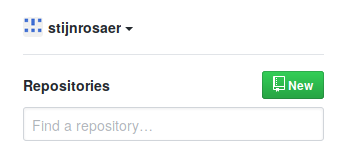
\includegraphics[scale=0.3]{img/maakrepo}\\ vul de nodige gegevens in\\ 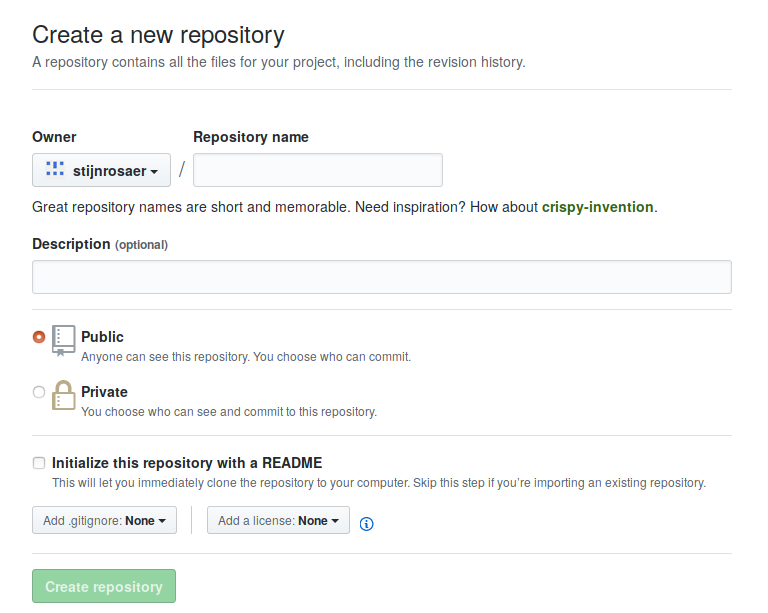
\includegraphics[scale=0.2]{img/maakrepo2}
					\item Voeg je ofline repository toe aan github:\\ \textit{git remote add origin [url van je github repository]}.
				\end{enumerate}
				
				\item Voeg hetgeen je op je pc hebt staan toe op github:\\ git push
				
				\item Download de wijzigingen op github:\\ \textit{git pull}
			\end{itemize}
			
			Een samenvatting en extra features kan je vinden op:\\ \href{https://services.github.com/on-demand/downloads/github-git-cheat-sheet.pdf}{\textit{https://services.github.com/on-demand/downloads/github-git-cheat-sheet.pdf}}
		
		\subsection{Github in PyCharm/CLion}
		\begin{enumerate}
			\item in terminal:\\ \textit{git clone [repository url]}
			\item Maak nu een nieuw project met de map die je juist gecloned hebt aan en klik op JA, dat je de bestanden wilt vervangen
			
			\item Gebruik de blauwe pijl om wijzigingen op te halen en de groene om er zelf door te voeren \\
			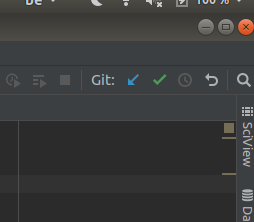
\includegraphics[scale=0.3]{img/pushpull}
			
			\item Voor het toevoegen moet je nog een message geven en zeker niet vergeten om commit en push te kiezen ipv commit
			\item gebruik de toetsencombinatie CTRL + SHIFT + TAB om te terminal te openen in PyCharm of CLion

		\end{enumerate}
		
		\subsection{Github rules}
		\begin{enumerate}
			\item push pas wanneer je code compileert, comitten kan je al eerder doen aangezien dit enkel op je computer komt.
			\item gebruik veel git status om te kijken wat er te gebeuren staat (voor git push, git pull, git commit, git add).
			\item pull eerst steeds vooraleer je pusht.			
			\item breek alles op in kleine stukjes (telkens er iets werkt commit en push je dit).
			\item doe NOOIT "git add ." vooraleer je git status gedaan hebt!
		\end{enumerate}
		
		\subsection{.gitignore file}
			De .gitignore file zorgt ervoor dat niet alle files meer toegevoegd worden. Hier kan je zelf nog extra extenties of files toevoegen. Git zal op deze manier bepaalde files niet mee comitten.
		\pagebreak
	
	
\includegraphics[scale=0.4]{img/github.png}
	\section{Exercise}
	\href{https://classroom.github.com/g/7nkanOf-}{\textit{https://classroom.github.com/g/7nkanOf-}}
		\subsection{Maak een repository aan en start een project}
			\begin{enumerate}
				\item (Persoon 1) ga naar de link en maak een groep aan
				\item (Persoon 2) ga naar de link en join het team van je groepspartner
				\item (Persoon 1\&2) kopieer de url
				\item (Persoon 1\&2) open een terminal en typ "git clone" en doe CTRL + SHIFT + V. De repository wordt nu gedownload op je pc.
			\end{enumerate}
		\subsection{gitignore}
			\emph{(Persoon 1\&2) Maak een python project met de gegeven bestanden.}
			
			\begin{enumerate}
				\item 1 iemand maakt een .gitignore file. Kijk via git status wat je niet wil toevoegen en zet dit in de file. 
				\item deze persoon doet een commit met een gepaste beschrijving en een push
				\item de andere persoon doet een pull. Kijk wat er is veranderd.
			\end{enumerate}
		\subsection{project}
			\begin{enumerate}
				\item Open beide je project.
				\item Eén persoon vervolledigd de fibonacci functie, de andere maakt factorial.
				\item Zorg dat je beide de twee functies hebt door gebruik te maken van push, pull en commit
				
				\item Pas beide in dezelfde functie hetzelfde aan, en push beide.
				\item Je krijgt nu een merge conflict omdat je beide hetzelfde aangepast hebt. Los dit op!		
			\end{enumerate}			
\end{document}

